\documentclass{beamer}

\usepackage{graphicx}

\usetheme{Boadilla}
\title{Memorization in Attention-only Transformers}
\author{Léo Dana}
\date{\today}

\begin{document}

\begin{frame}
    \titlepage
\end{frame}

\begin{frame}
    \frametitle{Memorization in Transformers}
    It is traditionnaly thought that MLP store information in Transformers.
    \begin{figure}
        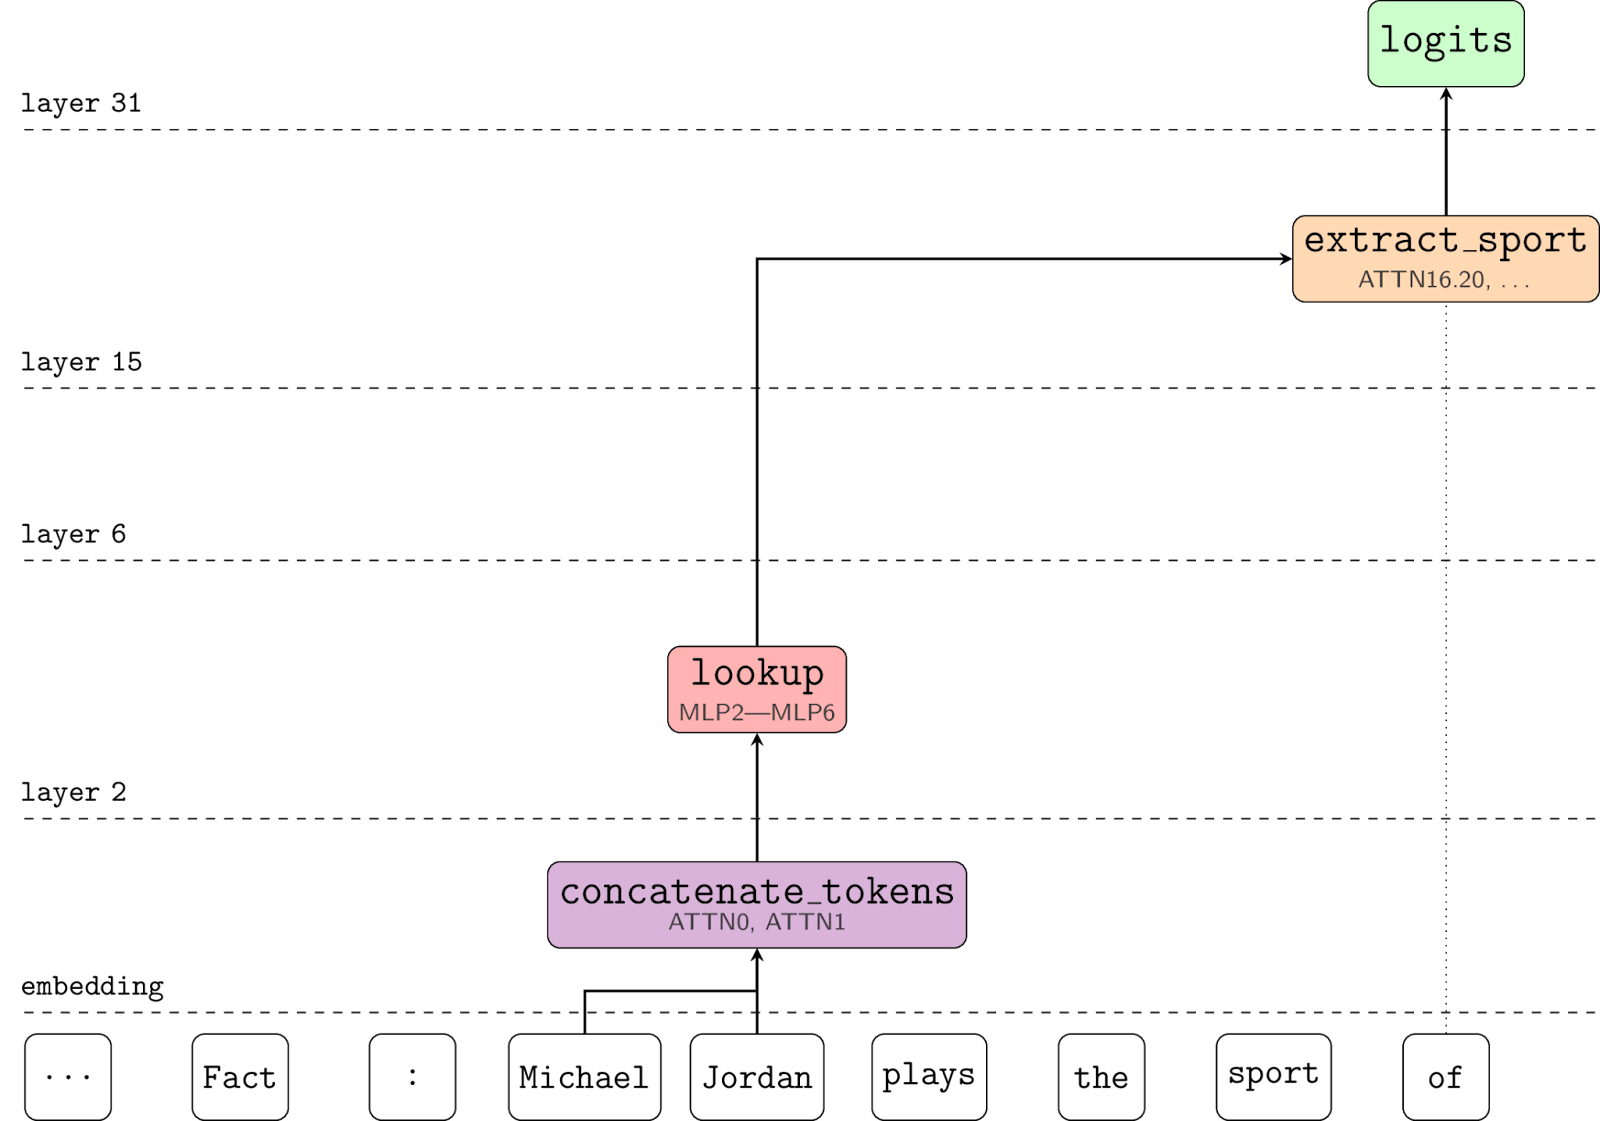
\includegraphics[width=0.7\textwidth]{./Look_up_table.png}
        \caption{From \textit{Fact Finding: Attempting to Reverse-Engineer Factual Recall on the Neuron Level}}
    \end{figure} 
\end{frame}

\begin{frame}
    \frametitle{Memorization in Transformers}
    We want to complete this view: maybe Attention layers can remember information. \\
    The questions we have begun to answer are:
    \begin{itemize}
        \item Can an Attention-only Transformer memorize ? How well can it do ?
        \item How much can it memorize ?
        \item How does it memorize ? What algorithm is implemented ?
    \end{itemize}
\end{frame}

\begin{frame}
    \frametitle{Associative memory}
    In \textit{Birth of a Transformer: A Memory Viewpoint. Bietti et al. 2023}, the Associative memory framework is introduced to Transformers.
    \break
    
    Goal: remember a mapping $g:[N]\rightarrow[N]$ using the argmax of $W_UWW_E$, where $W_U, W_E\in\mathbb{R}^{N,d}$ random embedding matrices,
    and $W\in\mathbb{R}^{d,d}$ is to learn.
    \break

    Using \[W = \sum_i w_U(g(i))^Tw_e(i)\] they show the model can remember association, but only $d$ of them.
\end{frame}

\begin{frame}
    \frametitle{Attention-only Transformers}
    \begin{figure}
        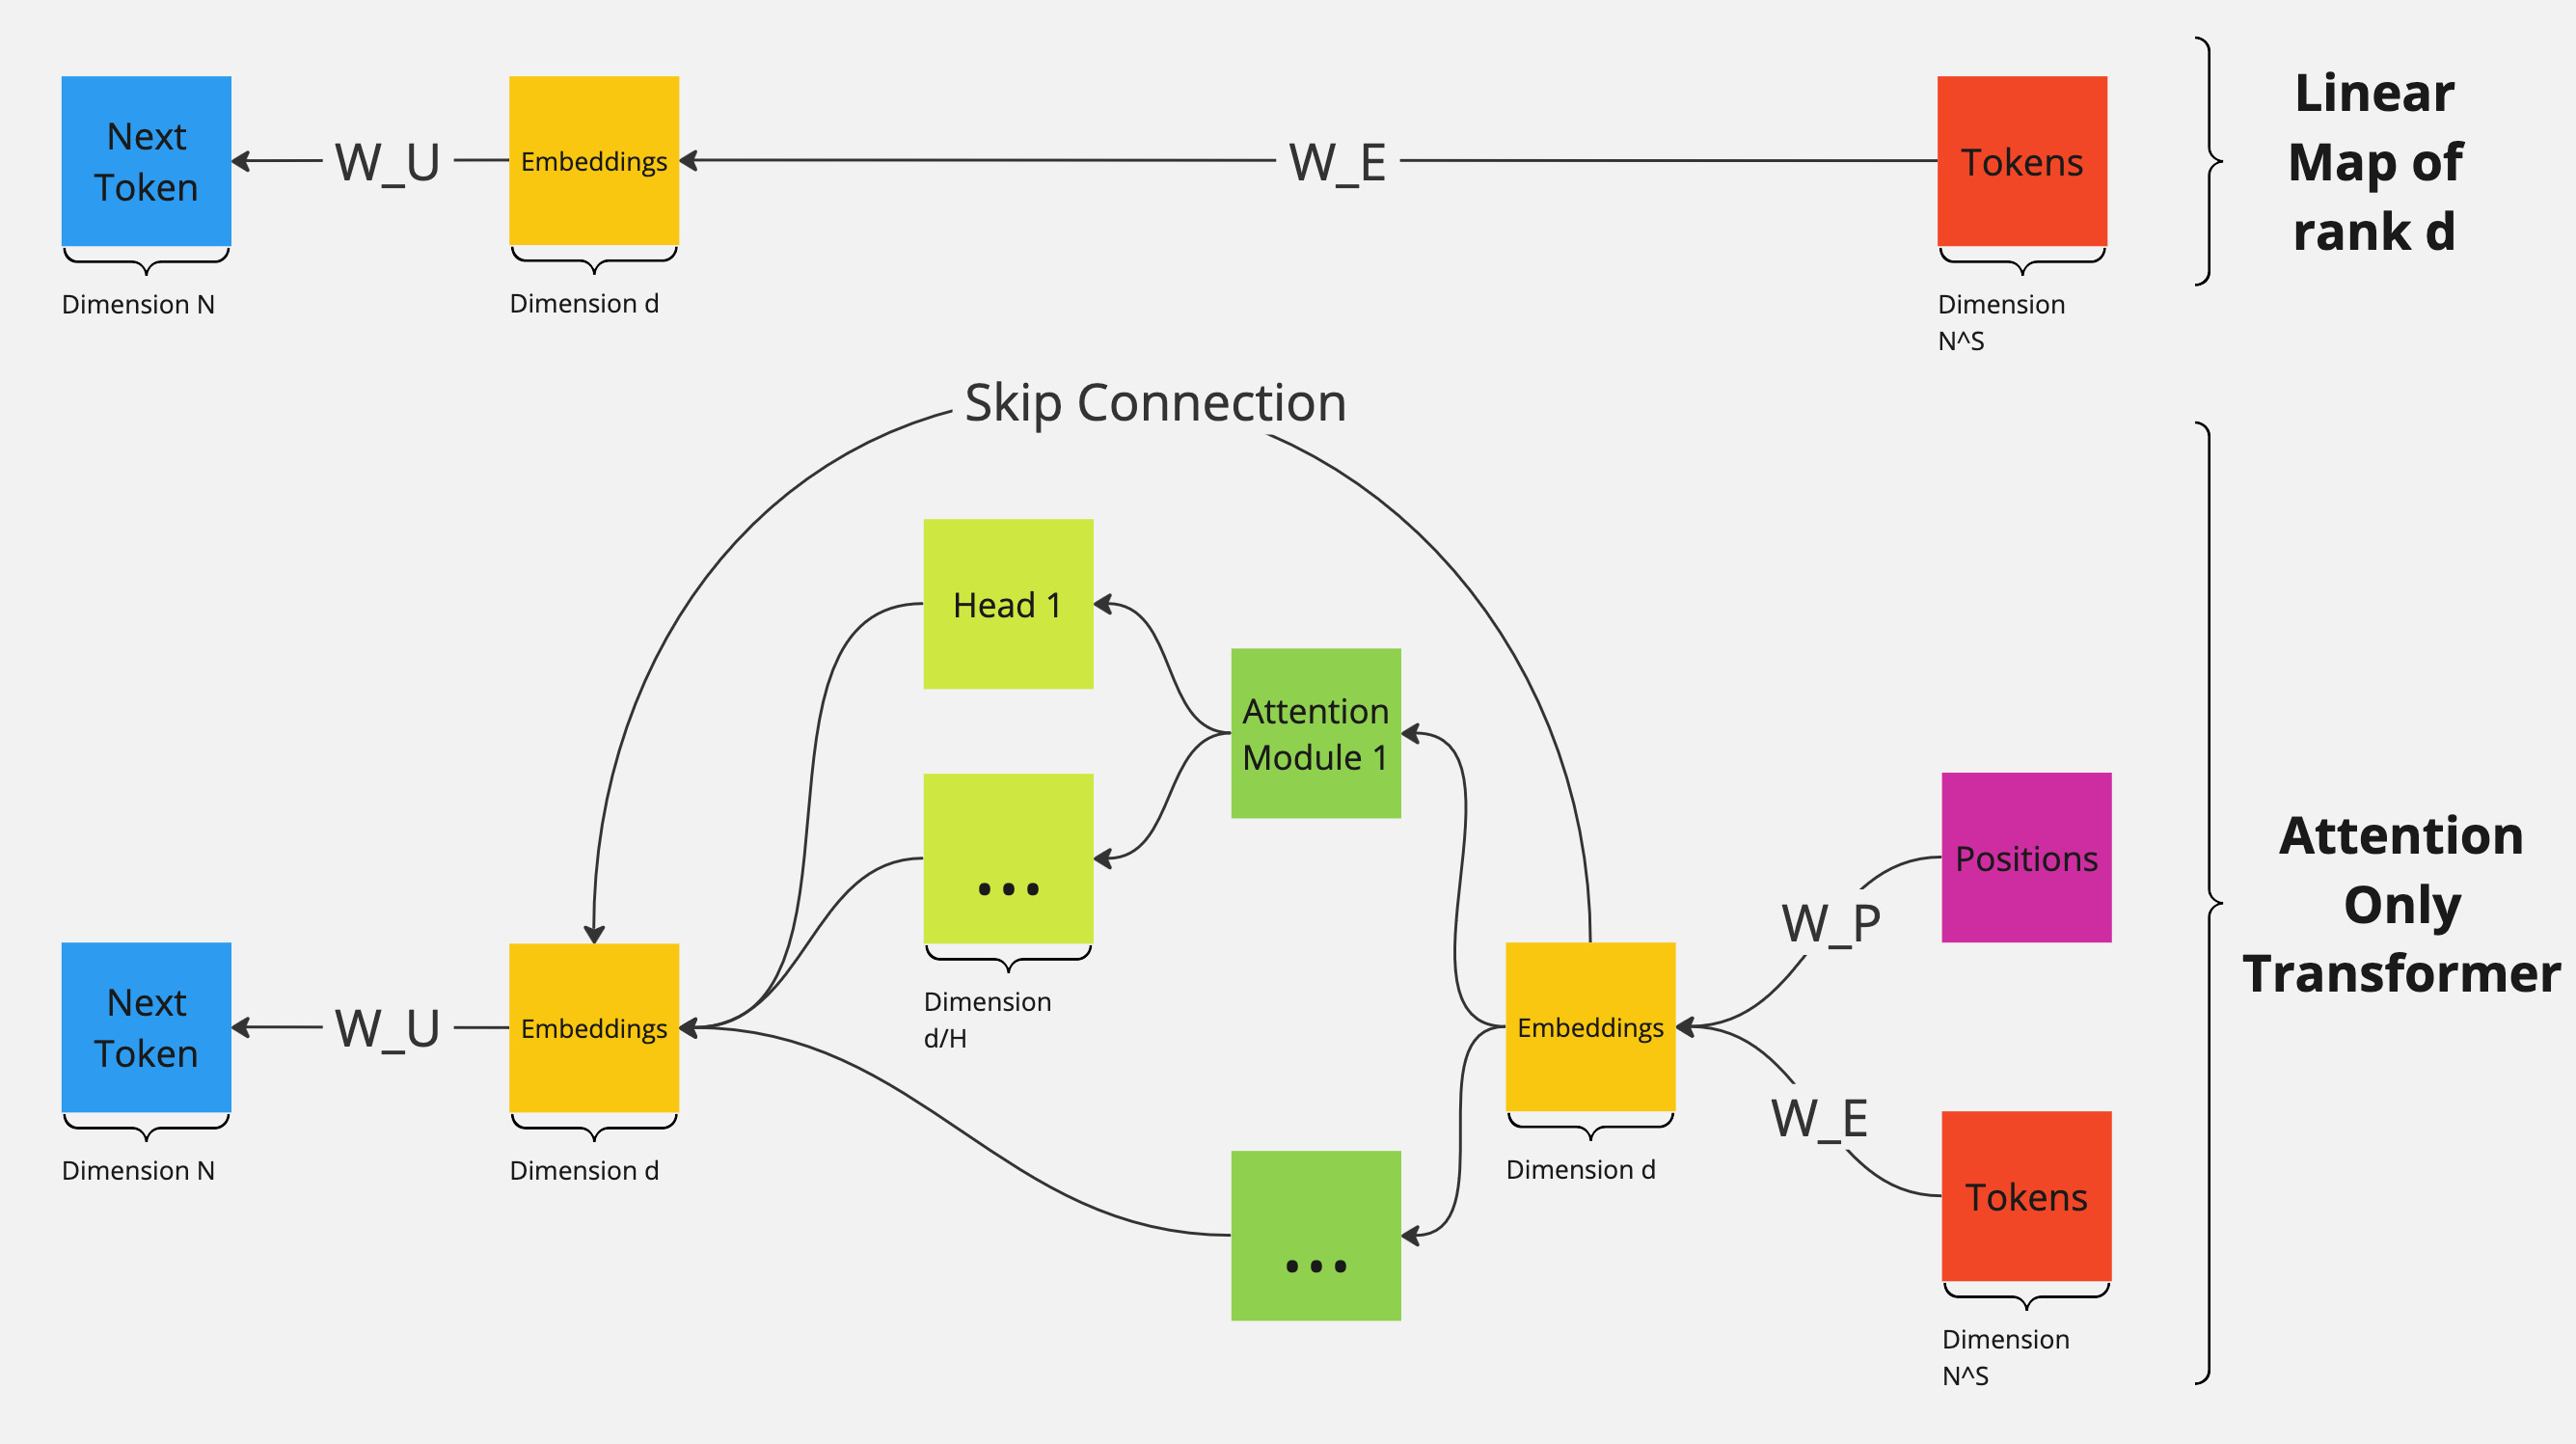
\includegraphics[width=\textwidth]{Transformer view 3.jpg}
    \end{figure}
\end{frame}

\begin{frame}
    \frametitle{Attention-only Transformers}
    Goal: memorize a distribution $\pi(t_{S+1}|t_S,...,t_1)$ for all sequences.
    \break

    \begin{theorem}
        Let $\varepsilon \geq 0$, $N_{\varepsilon}$ the smallest number of questions whose cumulative probability is greater than $1-\varepsilon$, 
        and $f_{W^*}$ the optimal linear mapping of rank $d$. \\
        There exist a transformer $T^*$ with embedding dimension $d$, $\left\lceil\frac{N_{\varepsilon}}{d}\right\rceil$ total parallel attention module 
        such that whose divergence with $\pi$ is
        \[\left|d_{KL}(\pi, f_{W^*}) - d_{KL}(\pi, T^*)\right| \leq \varepsilon\sigma_1(f_{W^*})C(d, N, k, N_{\varepsilon})\]
    \end{theorem}
\end{frame}

\begin{frame}
    \frametitle{Optimal Linear Mapping}
    Now we want to bound the quantity $d_{KL}(\pi, f_{W^*})$ to obtain an upper bound on the best Transformer possible.
    \[d_{KL}(\pi, T^*) \leq d_{KL}(\pi, f_{W^*})+\varepsilon\sigma_1(f_{W^*})C(d, N, k, N_{\varepsilon})\]

    \break

    We can acheive $0$ divergence if \[w_U(t_{S+1})^Tw_E(t_{1:S}) = \log(\pi(t_{S+1}|t_{1:S}))\] so if $L=\log(\pi)$ has rank $d$.\\
    \pause
    If $d\geq N-1$ this is always the case. Otherwise we look at special cases.
    \end{frame}

\begin{frame}
    \frametitle{Almost rank $d$}
    When the distribution to predict has low rank, a Taylor on the divergence reveals two possible optimal mappings:
    \pause
    \begin{itemize}
        \item $f_{ls}$ solution to the least-square problem \[||W_{ls} - L||_2\] 
        \[d_{KL}(\pi, f_{ls}) \leq N||\pi||_{+\infty}^2\sigma_{d+1}^2
        + (N||\pi||_{+\infty})^{\frac{3}{2}}\sigma_{d+1}^3\]
        \pause
        \item $f_{wls}$ solution to the weighted least-square problem \[||I_{\sqrt{\pi}}(W_{wls} - L)||_2\]
        \[d_{KL}(\pi, f_{wls}) \leq ||\pi||_{+\infty}\sigma_{d+1}^2
        + \left(\frac{||\pi||_{+\infty}}{||\pi||_{-\infty}}\right)^{\frac{3}{2}}\sigma_{d+1}^3\]
    \end{itemize}
    
\end{frame}

\begin{frame}
    \frametitle{Low Entropy}
    For low entropy, or look-up table, there exist a function $g:[N^S]\rightarrow[N]$ such that
    $\pi(t|t_{1:S}) \simeq \delta_{t=g(t_{1:S})}$.
    \pause
    \begin{figure}
        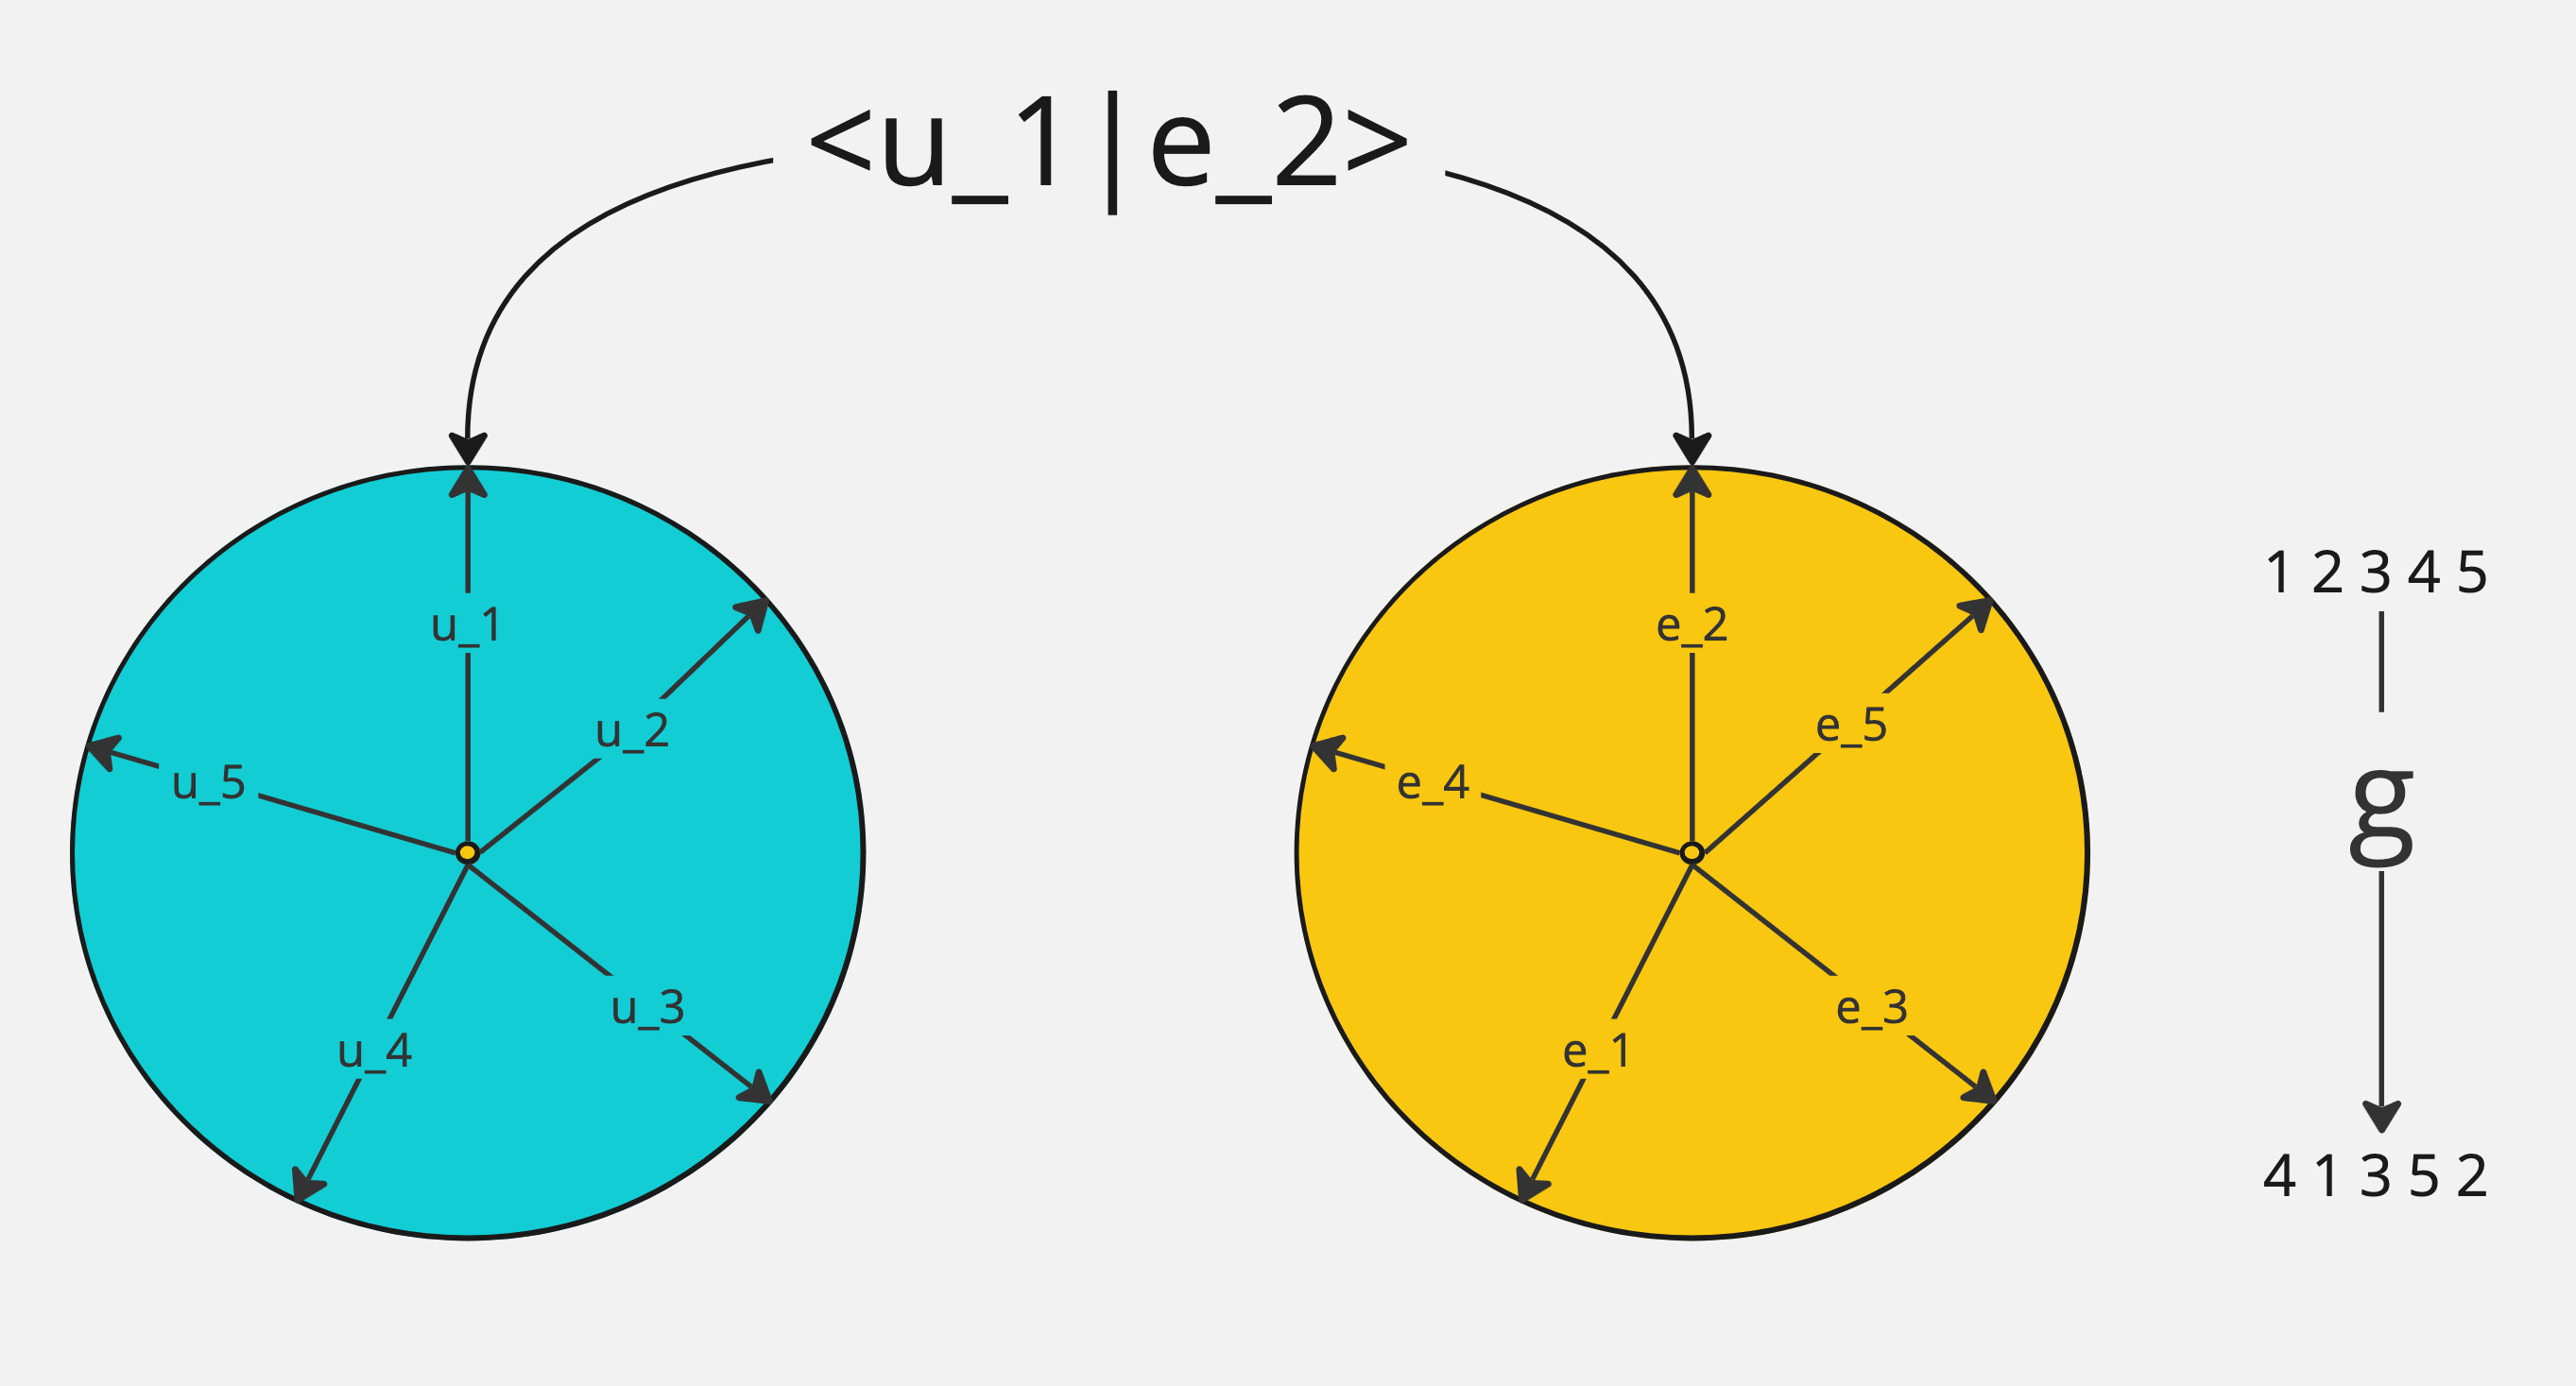
\includegraphics[width = 0.85\textwidth]{Low entropy.jpg}
    \end{figure}

\end{frame}

\begin{frame}
    \frametitle{Bound on the divergence}
    \begin{theorem}
        For this choice of $f$ and $C = \sqrt{\frac{32\log(N+1)}{d}}$, we have the bound
        \begin{equation*}
            \begin{split}
                d_{KL}(\pi, f) \leq \mathbb{E}_{t_{1:S}}\left[(1-\pi(g(t_{1:S})|t_{1:S}))\log\left(\frac{N-1}{e^{-H(\pi_{t_{1:S}})}-1}\right) \right]\left(\frac{1+4C}{1-2C}\right)
            \end{split}
        \end{equation*}
    \end{theorem}
\end{frame}

\begin{frame}
    \frametitle{Conclusion}
    We showed that 
    \begin{itemize}
        \item the attention mechanism in Transformers can memorize,
        \item we can quantify the error in some best cases,
    \end{itemize}
    \bigbreak

    Limitations:
    \begin{itemize}
        \item We do not know how memorization occurs in the sparce regime $dP < N_{\varepsilon}$,
        \item We cannot identify memorization behavior in a real Transformer's attention layer, 
    \end{itemize}
\end{frame}

\begin{frame}
    \frametitle{Experimental validation}

    \begin{figure}
        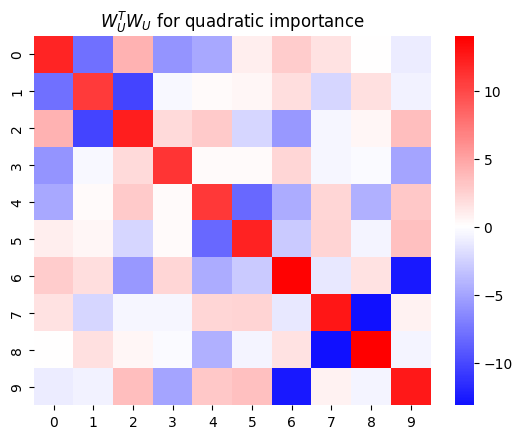
\includegraphics[width = 0.47\textwidth]{Uniform W_U.png}
        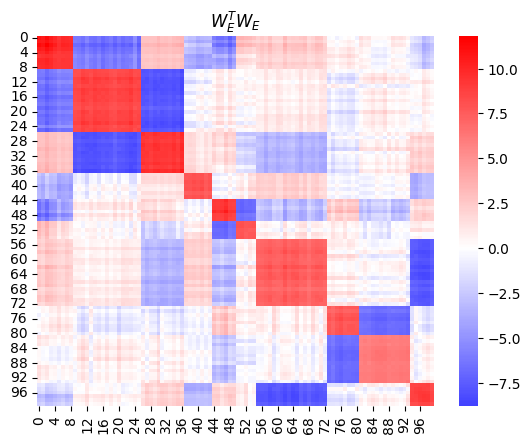
\includegraphics[width = 0.47\textwidth]{Uniform W_E.png}
    \end{figure}

    No memorization limit in term of quantity, but in term of quality !

\end{frame}

\end{document}